% !TEX root = ../thesis.tex
In the HEFT, two diagrams will be necessary to match that in Fig. \ref{hbb2l}. The first one is shown in Fig. \ref{HEFTgloop} and is the contribution that intuitively comes to mind when one thinks of integrating out top quarks from the SM diagrams.
The addition of the diagram of Fig. \ref{HEFTbbtree} is a necessity: the one-loop diagram alone is UV divergent and requires a counter-term.
We will indeed see that the $H\bbbar$ coupling of the HEFT has a counter-term proportional to $C_{\text{ggH}}$.
Besides this divergent term, matching the expanded SM calculation to these two diagrams will also show that a finite term needs to be absorbed in the $H\bbbar$ coupling to reproduce the SM, which is the term we have set out to obtain.

\begin{figure}[!h]
  \centering
  \subfloat[]{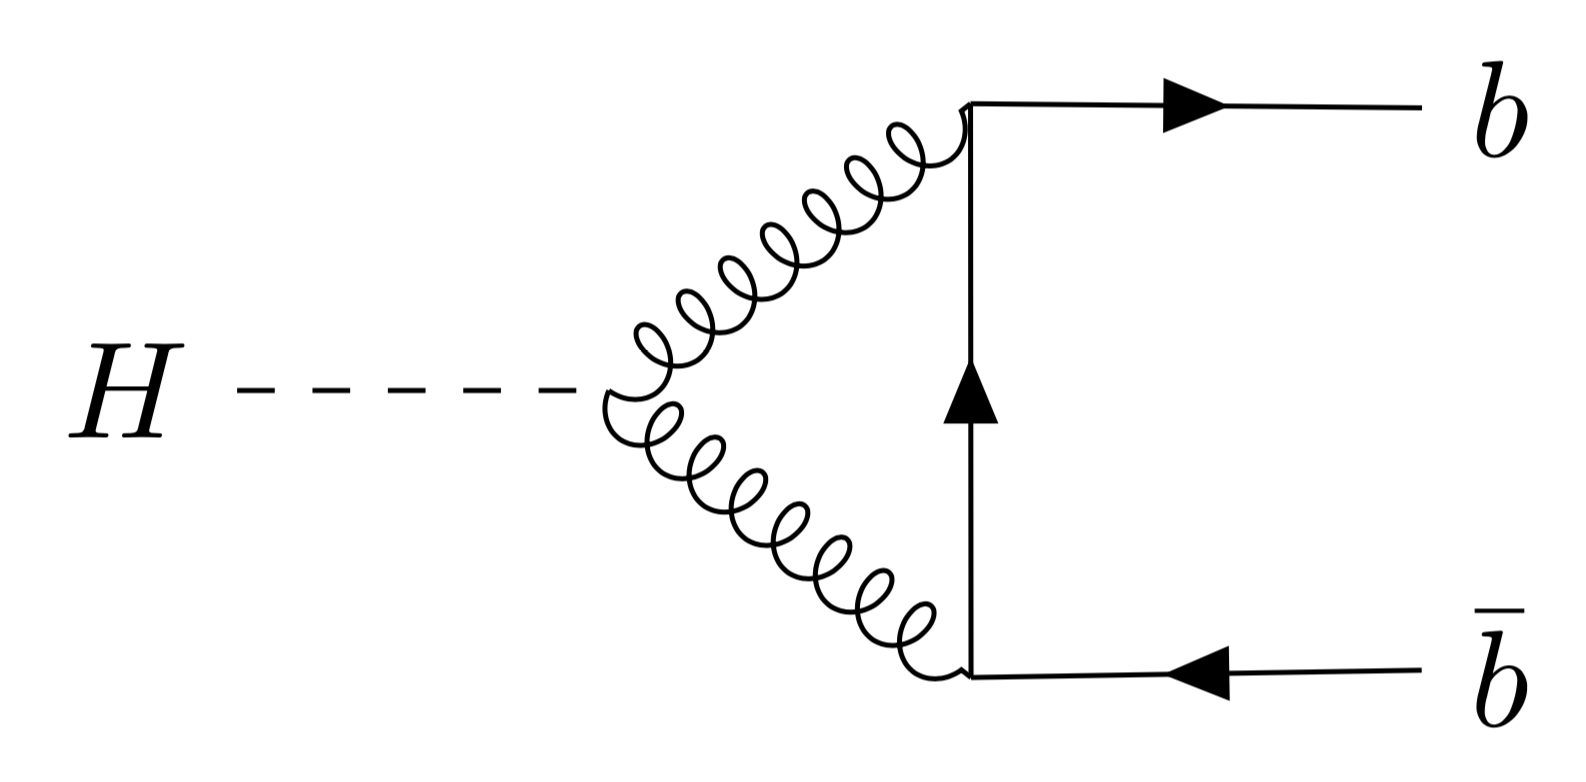
\includegraphics[height=7em]{Hbbgloop} \label{HEFTgloop}}\hspace{5em}
  \subfloat[]{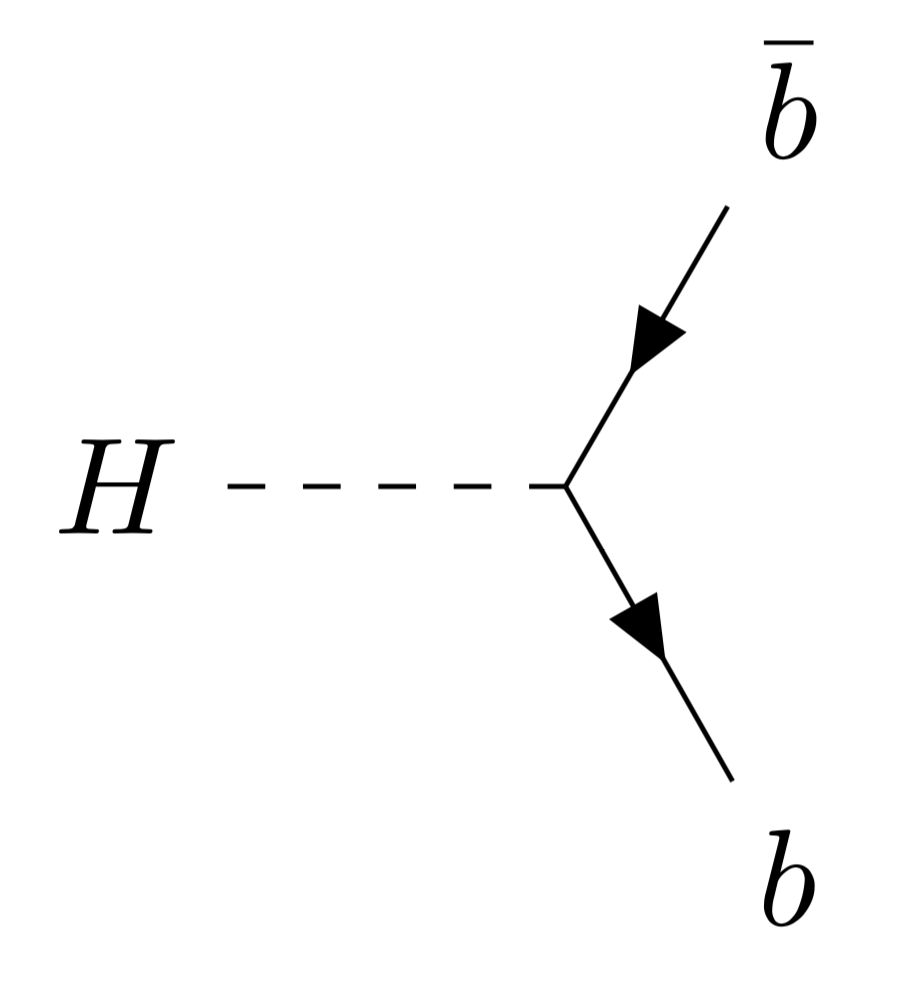
\includegraphics[height=8em]{Hbbtree}\label{HEFTbbtree}}\hspace{2em}
  \caption[$H\to\bbbar$ in the HEFT]{The two Feynman diagrams that contribute to $H\to \bbbar$ in the HEFT}
  \label{HEFThbbdiags}
\end{figure}

Another way to look at the presence of these two contributions will appear in the next section: the more complicated of the loop integrals that appear in the SM two-loop amplitude will have two regions in the $1/m_t$ expansion, which correspond to routing hard momenta through the top loop only or through the complete diagram.
These respectively have a diagramatical interpretation as shrinking the top loop in Fig. \ref{hbb2l} to obtain Fig. \ref{HEFTgloop} and shrinking the two loops to obtain Fig. \ref{HEFTbbtree}. This will be illustrated in the next section explicitly.

Since we wish to extract the power-suppressed corrections to a coupling that is present in the standard model, it is important that our notation makes a proper separation between the couplings in the SM and the HEFT to avoid confusion.
The interactions relevant for our calculation are the following:

\begin{table}[!h]
\begin{equation*}
{
  \renewcommand*{\arraystretch}{1.5}
  \begin{array}{cc}
    \toprule
    \text{Coupling} & \text{Value}\\\midrule
     {\cal L}_{y_b} = - \frac{C_{y_b}}{\sqrt{2}}h\bar b b; &C_{yb}=y_b+{\cal O}\left(\frac{1}{m_t}\right)\\
     {\cal L}_{Hgg} = -\frac{1}{4}C_{Hgg} G_{\mu\nu}G^{\mu\nu}h; & C_{Hgg}=\frac{\as}{3\pi v}\\
     {\cal L}_{bG} = i g_s G^\mu_a \bar b T^a\gamma_\mu b ; & \text{Fixed by gauge invariance}\\
    \bottomrule
\end{array}}
\end{equation*}
  \caption[HEFT Lagragian and couplings]{HEFT interactions relevant for the calculation of the ${\cal O}(g_s^4 y_t)$ contribution to $H\to \bar b b$ and their leading-order values in the $1/m_t$ expansion.}
  \label{HEFTcoupligs}
\end{table}

Taken as it is, the amplitude $\cala_1$ associated with the diagrams in Fig. \ref{HEFThbbdiags} has external spinor wavefunctions and can be written as $\cala_1 = \bar u_b^\sigma(p_1) \cala_1^\text{amp} v_{\bar b}^{\sigma'}(p_2)$.

Since this calculation is a means to the end of extracting a Wilson coefficient, we don't need the full information and can project and spin average $\cala_1$ to get rid of the spinors. In practice, we will therefore work with

\begin{equation}
  \cala = \sum_{\sigma\sigma'} \bar v_{\bar b}^{\sigma'}(p_2) u_b^\sigma(p_1) \cala_1
  =\text{Tr}\left((\not p_2-m_b)\cala_1^\text{amp}(\not p_1+m_b)\right).
\end{equation}
